
\documentclass[letterpaper,hide notes,xcolor={table,svgnames},pdftex]{beamer}
\def\showexamples{t}


%\usepackage[svgnames]{xcolor}

%% Demo talk
%\documentclass[letterpaper,notes=show]{beamer}

\usecolortheme{crane}
\setbeamertemplate{navigation symbols}{}

\usetheme{MyPittsburgh}
%\usetheme{Frankfurt}

%\usepackage{tipa}

\usepackage{hyperref}
\usepackage{graphicx,xspace}
\usepackage[normalem]{ulem}

\newcommand\SF[1]{$\bigstar$\footnote{SF: #1}}



\newcounter{tmpnumSlide}
\newcounter{tmpnumNote}

% old question code
%\newcommand\question[1]{{$\bigstar$ \small \onlySlide{2}{#1}}}
% \newcommand\nquestion[1]{\ifdefined \presentationonly \textcircled{?} \fi \note{\par{\Large \textbf{?}} #1}}
% \newcommand\nanswer[1]{\note{\par{\Large \textbf{A}} #1}}


 \newcommand\mnote[1]{%
   \addtocounter{tmpnumSlide}{1}
   \ifdefined\showcues {~\tiny\fbox{\arabic{tmpnumSlide}}}\fi
   \note{\setlength{\parskip}{1ex}\addtocounter{tmpnumNote}{1}\textbf{\Large \arabic{tmpnumNote}:} {#1\par}}}

\newcommand\mmnote[1]{\note{\setlength{\parskip}{1ex}#1\par}}

%\newcommand\mnote[2][]{\ifdefined\handoutwithnotes {~\tiny\fbox{#1}}\fi
% \note{\setlength{\parskip}{1ex}\textbf{\Large #1:} #2\par}}

%\newcommand\mnote[2][]{{\tiny\fbox{#1}} \note{\setlength{\parskip}{1ex}\textbf{\Large #1:} #2\par}}

\newcommand\mquestion[2]{{~\color{red}\fbox{?}}\note{\setlength{\parskip}{1ex}\par{\Large \textbf{?}} #1} \note{\setlength{\parskip}{1ex}\par{\Large \textbf{A}} #2\par}\ifdefined \presentationonly \pause \fi}

\newcommand\blackboard[1]{%
\ifdefined   \showblackboard
  {#1}
  \else {\begin{center} \fbox{\colorbox{blue!30}{%
         \begin{minipage}{.95\linewidth}%
           \hspace{\stretch{1}} Some space intentionally left blank; done at the blackboard.%
         \end{minipage}}}\end{center}}%
         \fi%
}



%\newcommand\q{\tikz \node[thick,color=black,shape=circle]{?};}
%\newcommand\q{\ifdefined \presentationonly \textcircled{?} \fi}

\usepackage{listings}
\lstset{%
  keywordstyle=\bfseries,
  aboveskip=15pt,
  belowskip=15pt,
  captionpos=b,
  identifierstyle=\ttfamily,
  escapeinside={(*@}{@*)},
  stringstyle=\ttfamiliy,
  frame=lines,
  numbers=left, basicstyle=\scriptsize, numberstyle=\tiny, stepnumber=0, numbersep=2pt}

\usepackage{siunitx}
\newcommand\sius[1]{\num[group-separator = {,}]{#1}\si{\micro\second}}
\newcommand\sims[1]{\num[group-separator = {,}]{#1}\si{\milli\second}}
\newcommand\sins[1]{\num[group-separator = {,}]{#1}\si{\nano\second}}
\sisetup{group-separator = {,}, group-digits = true}

%% -------------------- tikz --------------------
\usepackage{tikz}
\usetikzlibrary{positioning}
\usetikzlibrary{arrows,backgrounds,automata,decorations.shapes,decorations.pathmorphing,decorations.markings,decorations.text}

\tikzstyle{place}=[circle,draw=blue!50,fill=blue!20,thick, inner sep=0pt,minimum size=6mm]
\tikzstyle{transition}=[rectangle,draw=black!50,fill=black!20,thick, inner sep=0pt,minimum size=4mm]

\tikzstyle{block}=[rectangle,draw=black, thick, inner sep=5pt]
\tikzstyle{bullet}=[circle,draw=black, fill=black, thin, inner sep=2pt]

\tikzstyle{pre}=[<-,shorten <=1pt,>=stealth',semithick]
\tikzstyle{post}=[->,shorten >=1pt,>=stealth',semithick]
\tikzstyle{bi}=[<->,shorten >=1pt,shorten <=1pt, >=stealth',semithick]

\tikzstyle{mut}=[-,>=stealth',semithick]

\tikzstyle{treereset}=[dashed,->, shorten >=1pt,>=stealth',thin]

\usepackage{ifmtarg}
\usepackage{xifthen}
\makeatletter
% new counter to now which frame it is within the sequence
\newcounter{multiframecounter}
% initialize buffer for previously used frame title
\gdef\lastframetitle{\textit{undefined}}
% new environment for a multi-frame
\newenvironment{multiframe}[1][]{%
\ifthenelse{\isempty{#1}}{%
% if no frame title was set via optional parameter,
% only increase sequence counter by 1
\addtocounter{multiframecounter}{1}%
}{%
% new frame title has been provided, thus
% reset sequence counter to 1 and buffer frame title for later use
\setcounter{multiframecounter}{1}%
\gdef\lastframetitle{#1}%
}%
% start conventional frame environment and
% automatically set frame title followed by sequence counter
\begin{frame}%
\frametitle{\lastframetitle~{\normalfont(\arabic{multiframecounter})}}%
}{%
\end{frame}%
}
\makeatother

\makeatletter
\newdimen\tu@tmpa%
\newdimen\ydiffl%
\newdimen\xdiffl%
\newcommand\ydiff[2]{%
    \coordinate (tmpnamea) at (#1);%
    \coordinate (tmpnameb) at (#2);%
    \pgfextracty{\tu@tmpa}{\pgfpointanchor{tmpnamea}{center}}%
    \pgfextracty{\ydiffl}{\pgfpointanchor{tmpnameb}{center}}%
    \advance\ydiffl by -\tu@tmpa%
}
\newcommand\xdiff[2]{%
    \coordinate (tmpnamea) at (#1);%
    \coordinate (tmpnameb) at (#2);%
    \pgfextractx{\tu@tmpa}{\pgfpointanchor{tmpnamea}{center}}%
    \pgfextractx{\xdiffl}{\pgfpointanchor{tmpnameb}{center}}%
    \advance\xdiffl by -\tu@tmpa%
}
\makeatother
\newcommand{\copyrightbox}[3][r]{%
\begin{tikzpicture}%
\node[inner sep=0pt,minimum size=2em](ciimage){#2};
\usefont{OT1}{phv}{n}{n}\fontsize{4}{4}\selectfont
\ydiff{ciimage.south}{ciimage.north}
\xdiff{ciimage.west}{ciimage.east}
\ifthenelse{\equal{#1}{r}}{%
\node[inner sep=0pt,right=1ex of ciimage.south east,anchor=north west,rotate=90]%
{\raggedleft\color{black!50}\parbox{\the\ydiffl}{\raggedright{}#3}};%
}{%
\ifthenelse{\equal{#1}{l}}{%
\node[inner sep=0pt,right=1ex of ciimage.south west,anchor=south west,rotate=90]%
{\raggedleft\color{black!50}\parbox{\the\ydiffl}{\raggedright{}#3}};%
}{%
\node[inner sep=0pt,below=1ex of ciimage.south west,anchor=north west]%
{\raggedleft\color{black!50}\parbox{\the\xdiffl}{\raggedright{}#3}};%
}
}
\end{tikzpicture}
}


%% --------------------

%\usepackage[excludeor]{everyhook}
%\PushPreHook{par}{\setbox0=\lastbox\llap{MUH}}\box0}

%\vspace*{\stretch{1}

%\setbox0=\lastbox \llap{\textbullet\enskip}\box0}

\setlength{\parskip}{\fill}

\newcommand\noskips{\setlength{\parskip}{1ex}}
\newcommand\doskips{\setlength{\parskip}{\fill}}

\newcommand\xx{\par\vspace*{\stretch{1}}\par}
\newcommand\xxs{\par\vspace*{2ex}\par}
\newcommand\tuple[1]{\langle #1 \rangle}
\newcommand\code[1]{{\sf \footnotesize #1}}
\newcommand\ex[1]{\uline{Example:} \ifdefined \presentationonly \pause \fi
  \ifdefined\showexamples#1\xspace\else{\uline{\hspace*{2cm}}}\fi}

\newcommand\ceil[1]{\lceil #1 \rceil}


\AtBeginSection[]
{
   \begin{frame}
       \frametitle{Outline}
       \tableofcontents[currentsection]
   \end{frame}
}



\pgfdeclarelayer{edgelayer}
\pgfdeclarelayer{nodelayer}
\pgfsetlayers{edgelayer,nodelayer,main}

\tikzstyle{none}=[inner sep=0pt]
\tikzstyle{rn}=[circle,fill=Red,draw=Black,line width=0.8 pt]
\tikzstyle{gn}=[circle,fill=Lime,draw=Black,line width=0.8 pt]
\tikzstyle{yn}=[circle,fill=Yellow,draw=Black,line width=0.8 pt]
\tikzstyle{empty}=[circle,fill=White,draw=Black]
\tikzstyle{bw} = [rectangle, draw, fill=blue!20, 
    text width=4em, text centered, rounded corners, minimum height=2em]
    
    \newcommand{\CcNote}[1]{% longname
	This work is licensed under the \textit{Creative Commons #1 3.0 License}.%
}
\newcommand{\CcImageBy}[1]{%
	\includegraphics[scale=#1]{creative_commons/cc_by_30.pdf}%
}
\newcommand{\CcImageSa}[1]{%
	\includegraphics[scale=#1]{creative_commons/cc_sa_30.pdf}%
}
\newcommand{\CcImageNc}[1]{%
	\includegraphics[scale=#1]{creative_commons/cc_nc_30.pdf}%
}
\newcommand{\CcGroupBySa}[2]{% zoom, gap
	\CcImageBy{#1}\hspace*{#2}\CcImageNc{#1}\hspace*{#2}\CcImageSa{#1}%
}
\newcommand{\CcLongnameByNcSa}{Attribution-NonCommercial-ShareAlike}

\newenvironment{changemargin}[1]{% 
  \begin{list}{}{% 
    \setlength{\topsep}{0pt}% 
    \setlength{\leftmargin}{#1}% 
    \setlength{\rightmargin}{1em}
    \setlength{\listparindent}{\parindent}% 
    \setlength{\itemindent}{\parindent}% 
    \setlength{\parsep}{\parskip}% 
  }% 
  \item[]}{\end{list}} 




\title{Lecture 7 --- Android II}

\author{Patrick Lam\\ \small \texttt{p.lam@ece.uwaterloo.ca} }
\institute{Department of Electrical and Computer Engineering \\
  University of Waterloo}
\date{\today}
\begin{document}

\begin{frame}
  \titlepage
\end{frame}

\part{Programming Tips}
\frame{\partpage}

\begin{frame}
\frametitle{Programming Tips}
\begin{changemargin}{1cm}

First, a programming tip for object-oriented systems. 

Sometimes, you have code
in a class, say an {\tt EventListener}, which needs access to the object
that created it, say the {\tt MainActivity}. 

Add a field to the {\tt EventListener}
with a reference to the {\tt MainActivity}, as follows:

\end{changemargin}
\end{frame}

\begin{frame}[fragile]
\frametitle{Programming Tips}
\begin{changemargin}{0.5cm}

{\scriptsize \begin{verbatim}
    public class MainActivity extends Activity {
      @Override
      protected void onCreate(Bundle savedInstanceState) {
        // ...
        LightSensorEventListener el = new LightSensorEventListener(this);
      }
    }

    class LightSensorEventListener implements SensorEventListener {
      MainActivity m;

      public LightSensorEventListener(MainActivity m) {
        this.m = m;
      }

      // ...
    }
\end{verbatim}
}

\end{changemargin}
\end{frame}

\begin{frame}
\frametitle{Programming Tips}
\begin{changemargin}{1cm}

Don't put your app in the {\tt com.example} namespace. 

Put it in {\tt ca.uwaterloo}.
\end{changemargin}
\end{frame}

\part{Android Intents}
\frame{\partpage}

\begin{frame}
\frametitle{Intents}
\begin{changemargin}{1cm}

So far we only examined an Activity in isolation.

For the labs, you won't need anything more.

In real apps, there's usually multiple activities.

We link them with Intents.

\end{changemargin}
\end{frame}

\begin{frame}[fragile]
\frametitle{Intents}
\begin{changemargin}{1cm}

An \emph{Intent} specifies a request or describes an event.

The simplest possible Intent
explicitly names the Activity it would like to start.

{\small 
\begin{verbatim}
  Intent intent = new Intent(this, OtherActivity.class);
  startActivity(intent);
\end{verbatim}
}


\end{changemargin}
\end{frame}


\begin{frame}
\frametitle{Intent: Request Example}
\begin{changemargin}{1cm}


The Map activity puts up links to webpages 
\& phone numbers. 

Upon click, the Map broadcasts either the web browser
Intent or the call Intent.

The Map trusts that some other application will handle the Intent.
\end{changemargin}
\end{frame}



\begin{frame}
\frametitle{Intent: Event Example}
\begin{changemargin}{.8cm}

The system broadcasts an Intent when the phone
enters flight mode.

\end{changemargin}
\end{frame}

\begin{frame}
\frametitle{How Intents Work}
\begin{changemargin}{1cm}
 One component broadcasts an Intent. 

Then, 0 or more components receive the Intent. 

Android may pick a component
to act upon the Intent.

\end{changemargin}
\end{frame}

\begin{frame}
\frametitle{Choosing the Handler}
\begin{changemargin}{1cm}
\begin{center}
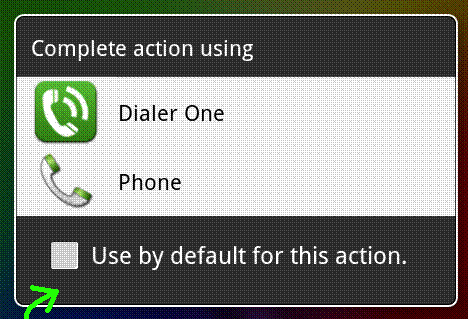
\includegraphics[height=.5\textheight]{images/completeaction.png}
\end{center}
(Image from stackoverflow.com)

In this case, the user is asked to choose.

\end{changemargin}
\end{frame}


\begin{frame}
\frametitle{Parts of an Intent}
\begin{changemargin}{1cm}

Each intent contains an \emph{action} which represents the requested
action, along with optional data. For instance:

\hspace*{2em} \begin{tabular}{ll}
ACTION\_MAIN & Launch an activity \\
ACTION\_DIAL & Dial a phone number \\
ACTION\_SEARCH & Perform a search
\end{tabular}

\end{changemargin}
\end{frame}


\begin{frame}[fragile]
\frametitle{Parts of an Intent}
\begin{changemargin}{1cm}

The two following code fragments yield identical Intents with an action (but no data):

\end{changemargin}
{\scriptsize
\begin{verbatim}
new Intent(Intent.ACTION_EDIT);   |  Intent intent = new Intent();
                                  |  intent.setAction(Intent.ACTION_EDIT);
\end{verbatim}
}



\end{frame}


\begin{frame}
\frametitle{Parts of an Intent}
\begin{changemargin}{1cm}

The \emph{data} is the payload of the event. 

Android intent data is in
URI (Universal Resource Identifier) format\footnote{What's a URI? It's
  like a URL. The exact distinction is unimportant for ECE155.}. 
  
  The
obvious thing to put into data is a web address, but other data formats
are possible as well:

\end{changemargin}
\end{frame}


\begin{frame}[fragile]
\frametitle{Parts of an Intent}
{\scriptsize
\begin{verbatim}
new Intent(Intent.ACTION_DIAL,           | Intent intent = 
                                         |   new Intent(Intent.ACTION_DIAL);
           Uri.parse("tel:6175551212")); | intent.setData(
                                         |   Uri.parse("tel:6175551212"));
\end{verbatim}
}
\end{frame}


\begin{frame}
\frametitle{Parts of an Intent}
\begin{changemargin}{1cm}

You can also tell Android what type of data to expects.

Use the {\tt setType} method. Example: {\tt
  intent.setType("audio/mp3");}

This is optional. 


\end{changemargin}
\end{frame}



\begin{frame}
\frametitle{Intent Extras}
\begin{changemargin}{1cm}

Beyond the data, Intents may also contain \emph{extras}. 

Extras
consist of key-value pairs. 

They contain more information than what
can easily be put in a URI.

\end{changemargin}
\end{frame}


\begin{frame}[fragile]
\frametitle{Intent Extras Example}
\begin{changemargin}{1cm}

{\small 
\begin{verbatim}
Intent intent = new Intent(Intent.ACTION_SEND);
intent.putExtra(android.content.Intent.EXTRA_EMAIL,
  new String[] {
    "p.lam@ece.uwaterloo.ca", "root@uwaterloo.ca"
  });
\end{verbatim}
}


\end{changemargin}
\end{frame}



\begin{frame}
\frametitle{Intent Flags}
\begin{changemargin}{1cm}

Finally, Intents may also contain \emph{flags}.

These modify how the
Intent gets launched and how it will be processed by the recipient. 


They don't affect which activity gets launched. 

Examples: {\tt FLAG\_ACTIVITY\_NO\_HISTORY} and 
{\tt FLAG\_ACTIVITY\_RESET\_TASK\_IF\_NEEDED}.

\end{changemargin}
\end{frame}


\begin{frame}
\frametitle{Intent Resolution}
\begin{changemargin}{1cm}
We've can explicitly name which Activity we want to launch.

We can implicitly launch an activity by
describing what we want. 

In either case, use {\tt
  startActivity}  to launch the intent.

Implicit intent resolution: system searches the
available Activities, using the Intent's action, data
and category.

\end{changemargin}
\end{frame}

\begin{frame}[fragile]
\frametitle{Requesting Intent Resolution}
\begin{changemargin}{1cm}

{\small 
\begin{verbatim}
  private static final int REQUEST_CODE = 1;

  public void pickImage(View View) {
    Intent intent = new Intent();
    intent.setType("image/*");
    intent.setAction(Intent.ACTION_GET_CONTENT);
    intent.addCategory(Intent.CATEGORY_OPENABLE);
    startActivityForResult(intent, REQUEST_CODE);
  }
\end{verbatim}
}


\end{changemargin}
\end{frame}

\begin{frame}[fragile]
\frametitle{Responding to Intent Resolution Requests}
\begin{changemargin}{1cm}

In your application's manifest, there's an XML tag for each activity.
That tag can take an \emph{intent filter} describing the Intents
that the activity is prepared to handle. For example:
{\scriptsize 
\begin{verbatim}
<activity
    android:name=".BrowserActivity"
    android:label="@string/app_name" >
    <intent-filter>
        <action android:name="android.intent.action.VIEW" />

        <category android:name="android.intent.category.DEFAULT" />

        <data android:scheme="http" />
    </intent-filter>
</activity>
\end{verbatim}
}
This activity is able to view any URI that begins with {\tt http}.


\end{changemargin}
\end{frame}

\begin{frame}[fragile]
\frametitle{Receiving Activity Results}
\begin{changemargin}{1cm}

When you launch a sub-Activity, sometimes you're hoping for a result
back from that activity. 

For instance, you may be asking for the
user to pick a contact from the contact list. 

Or you may be asking the
user for a favourite colour. 

The sub-activity should
create a new Intent and call its {\tt setResult} method:

{\scriptsize 
\begin{verbatim}
  Intent retval = new Intent();
  retval.putExtra("color", "blue");
  setResult(RESULT_OK, retval);
\end{verbatim}
}


\end{changemargin}
\end{frame}


\begin{frame}[fragile]
\frametitle{Receiving Activity Results}
\begin{changemargin}{1cm}

Then in the caller, we provide a new callback, {\tt onActivityResult()}.

{\scriptsize
\begin{verbatim}
  @Override
  protected void onActivityResult(int requestCode, 
                           int resultCode, Intent data) {
    if (resultCode == RESULT_OK && requestCode == YOUR_REQUEST_CODE) {
      if (data.hasExtra("color")) {
        String favouriteColor = data.getExtras().getString("color");
      }
   }
  }
\end{verbatim}
}

\end{changemargin}
\end{frame}

\begin{frame}[fragile]
\frametitle{Receiving Activity Results}
\begin{changemargin}{1cm}


The {\tt resultCode} is an {\tt int} you provided while starting the
sub-activity. 

It allows you to distinguish different sub-activities you
may have started.



\end{changemargin}
\end{frame}


\begin{frame}
\frametitle{Passing Data Using Intents}

Video:\\
\url{https://www.youtube.com/watch?v=0ism1OM0an0}

\end{frame}


\part{Saving \& Restoring State}
\frame{\partpage}

\begin{frame}
\frametitle{Saving and Restoring State}
\begin{changemargin}{1cm}
Sometimes, Android kills your activity but brings it back later.

You want the activity to have the same data when it comes back from the
dead.

This will happen by default for anything in a UI element, but
not for any fields stored in the activity (like, say, step counts).

In your activity, implement the callback {\tt onSaveInstanceState()}

\end{changemargin}
\end{frame}


\begin{frame}[fragile]
\frametitle{Saving State}

\begin{changemargin}{1cm}
 To save state:
 
(The Bundle {\tt b} is another key/value map.)
 


{\scriptsize
\begin{verbatim}
class MainActivity ... {
  String color;

  @Override
  protected void onSaveInstanceState(Bundle b) {
    super.onSaveInstanceState(b);
    b.putString("color", color);
  }
}
\end{verbatim}
}
\end{changemargin}
\end{frame}


\begin{frame}[fragile]
\frametitle{Restoring State}

\begin{changemargin}{1cm}
 You can then restore whatever data you saved in the {\tt onCreate} method of the same Activity:

{\scriptsize
\begin{verbatim}
class MainActivity ... {
  @Override
  protected void onCreate(Bundle savedInstanceState) {
    if (savedInstanceState != null)
      color = b.getString("color");
  }
}
\end{verbatim}
}
\end{changemargin}
\end{frame}


\part{Graphics on Android}
\frame{\partpage}

\begin{frame}
\frametitle{XML versus Programmatic Construction}

\begin{changemargin}{1cm}
Use the right tool for the job!\\[1em]

XML = more safety:
\begin{itemize}
\item Select and place items ahead of time.
\item Don't need the emulator to see how things will look.
\item More error checking.
\end{itemize}
~\\

Java Code = more flexibility:
\begin{itemize}
\item Can choose widgets based on user input or computations.
\item Can use loops, etc to generate related items.
\item Less error checking.
\end{itemize}

\end{changemargin}
\end{frame}

\begin{frame}[fragile]
\frametitle{What ``inflate'' means}

\begin{changemargin}{1cm}
These lines keep on showing up in our code:
{\scriptsize
\begin{verbatim}
// Inflate the menu; this adds items to the 
// action bar if it is present.
getMenuInflater().inflate(R.menu.activity_main, menu);
\end{verbatim}
}

``Inflate'' = taking an XML and\\
 creating {\tt View} objects, based
on the description in the XML.
\end{changemargin}
\end{frame}

\begin{frame}[fragile]
\frametitle{Putting Graphics on the Screen}
\begin{changemargin}{1cm}
Two choices:
\begin{itemize}
\item use a {\tt View} (easier; infrequent updates); or
\item paint to a {\tt Canvas} (more complicated, many updates).
\end{itemize}
\end{changemargin}
\end{frame}

\begin{frame}[fragile]
\frametitle{Main class: {\tt Drawable}}
\begin{changemargin}{1cm}
Represents ``something that can be drawn'', e.g.
\begin{itemize}
\item BitmapDrawable
\item ShapeDrawable
\item PictureDrawable
\item etc.
\end{itemize}
\end{changemargin}
\end{frame}


\begin{frame}[fragile]
\frametitle{Drawing to a View}
\begin{changemargin}{1cm}
As always with Android, either:
\begin{itemize}
\item through XML; or
\item programmatically.
\end{itemize}
\end{changemargin}
\end{frame}

\begin{frame}[fragile]
\frametitle{Bitmaps through ImageView}

\begin{changemargin}{1cm}
Easiest way\footnote{Thanks to \scriptsize \url{http://www.cs.umd.edu/class/fall2010/CMSC498G/CMSC498G/Slides_files/Graphics.pptx}}: 
\begin{itemize}
\item put a picture ({\tt PNG}, {\tt JPG} or {\tt GIF}) in {\tt res/drawables}.
\item use an {\tt ImageView} to include it on the screen.
\end{itemize}


{\tiny from: \url{http://developer.android.com/guide/topics/graphics/2d-graphics.html}}

{\scriptsize
\begin{verbatim}
  // Instantiate an ImageView and define its properties programmatically
  ImageView i = new ImageView(this);
  i.setImageResource(R.drawable.my_image);
   // set the ImageView bounds to match the Drawable's dimensions
  i.setAdjustViewBounds(true);
  i.setLayoutParams(new Gallery.LayoutParams
      (LayoutParams.WRAP_CONTENT, LayoutParams.WRAP_CONTENT));

  // Add the ImageView to the layout and 
  //  set the layout as the content view
  mLinearLayout.addView(i);
\end{verbatim}
}
\end{changemargin}
\end{frame}


\begin{frame}[fragile]
\frametitle{Bitmaps through ImageView XML}

\begin{changemargin}{1cm}
Again, you need the appropriate drawable in the {\tt res/drawables} directory.\\[1em]
Note: harder to go wrong here.

\begin{verbatim}
  <ImageView
    android:id="@+id/imageView1"
    android:layout_height="wrap_content"
    android:layout_width="wrap_content"
    android:src="@drawable/myImage" />
\end{verbatim}

\end{changemargin}

\end{frame}

\begin{frame}[fragile]
\frametitle{Drawing on a ShapeDrawable}
\begin{changemargin}{1cm}
Primitive shapes: 
\begin{itemize}
\item PathShape---lines;
\item RectShape---rectangles;
\item OvalShape---ovals and rings;
\end{itemize}
Once again, we put these into an {\tt ImageView}.
\end{changemargin}
\end{frame}

\begin{frame}[fragile]
\frametitle{Shapes from XML}

\begin{changemargin}{1cm}
Again, you need the appropriate drawable in the {\tt res/drawables} directory.\\[1em]
Note: harder to go wrong here.

In the Layout XML:
\begin{verbatim}
  <ImageView android:id="@+id/imageView2"
    android:src="@drawable/cyan_shape" ... />
\end{verbatim}

Next, we create an XML for the drawable itself:
\begin{verbatim}
  <shape android:shape="oval" ... >
    <size android:width="160px" 
    	android:height="160px" />
    <solid android:color="#7f00ffff" />
  </shape>
\end{verbatim}

\end{changemargin}
\end{frame}

\begin{frame}[fragile]
\frametitle{Shapes, programmatically}
\begin{changemargin}{1cm}
Everything you can do in XML, you can do in code.

{\scriptsize
\begin{verbatim}
  private class MyDrawableView extends ImageView {
    private ShapeDrawable mDrawable;
    public MyDrawableView(Context context, int color) {
      ...
      mDrawable = new ShapeDrawable(new OvalShape());
      mDrawable.getPaint().setColor(color);
      mDrawable.setBounds(0, 0, size, size);
      mDrawable.setAlpha(alpha);
    }
    protected void onDraw(Canvas canvas) {
      mDrawable.draw(canvas);
    }
  }
\end{verbatim}
}

\end{changemargin}
\end{frame}

\begin{frame}[fragile]
\frametitle{Shapes, programmatically}
\begin{changemargin}{1cm}
In the Activity's {\tt onCreate()}:
\begin{verbatim}
  MyDrawableView magentaView = 
    new MyDrawableView(this, Color.MAGENTA);
  magentaView.setLayoutParams
    (new LinearLayout.LayoutParams(160, 160));
  addView(magentaView);
\end{verbatim}
\end{changemargin}
\end{frame}

\begin{frame}
\frametitle{9-patches}

\begin{changemargin}{1cm}

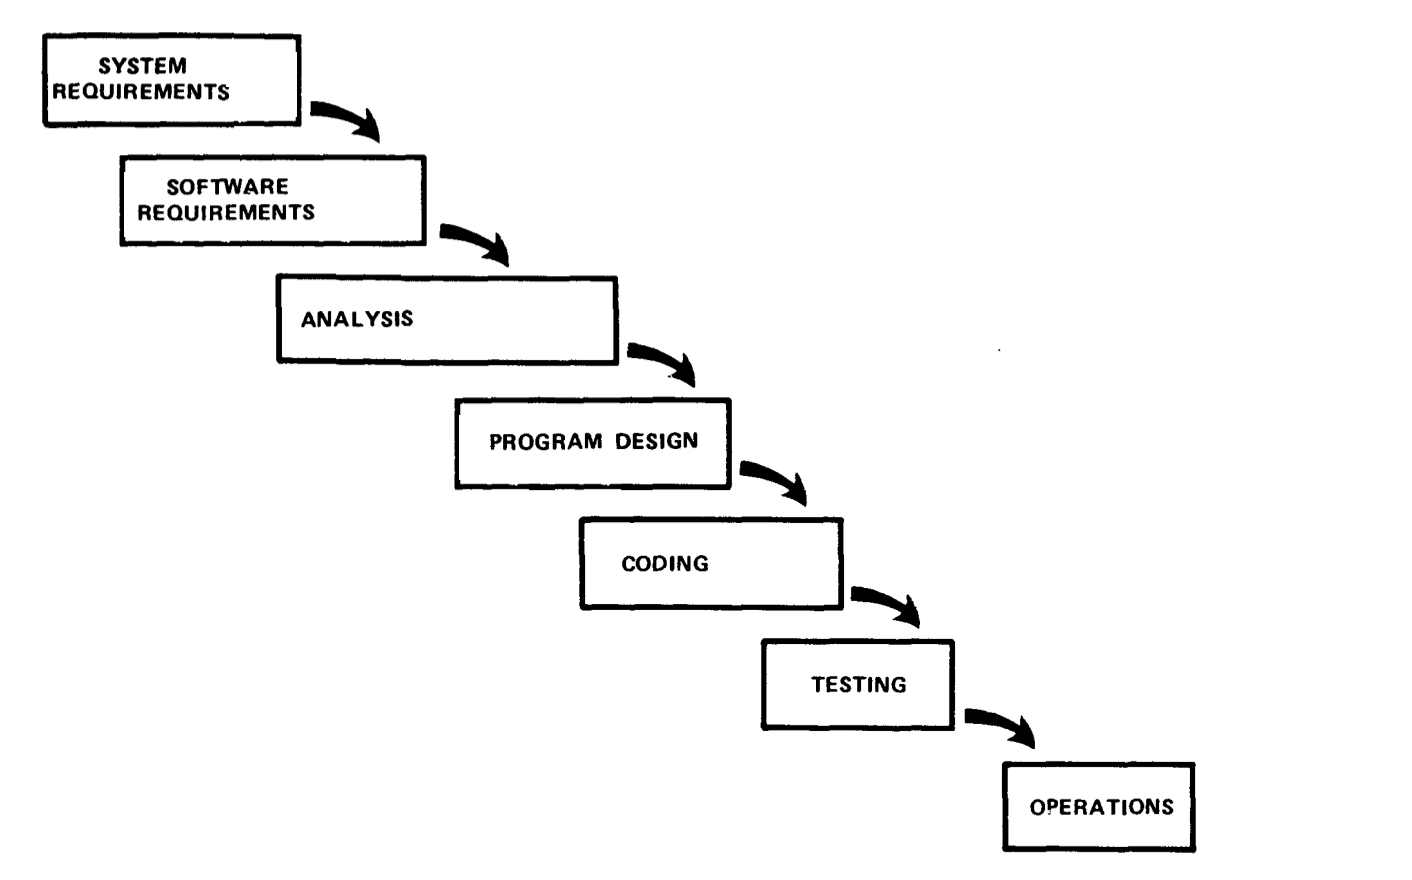
\includegraphics[height=.7\textheight]{images/concurrent-engineering.png}

I manually stretched the boxes using a graphics editor.\\[1em]

\end{changemargin}
\end{frame}

\begin{frame}
\frametitle{9-patches: automatic stretching}

\begin{changemargin}{1cm}
{\tt NinePatchDrawable} can stretch your images automatically!

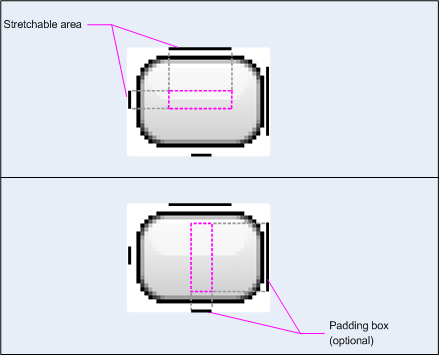
\includegraphics[height=.7\textheight]{images/ninepatch_raw}\\

Just use a {\tt .9.png} file.  Edit using {\tt tools/draw9patch}.
\end{changemargin}
\end{frame}





\end{document}
